\chapter{Theoretical and Technical Foundation}
\label{chap:theoretical_foundation}

This chapter presents the theoretical, legal, and technical foundation for \gls{SafeVision}. It defines sensitive information in visual media, outlines the \acrshort{gdpr}-related constraints that affect such data, and reviews redaction workflows,
AI-based methods, and the model choices used in the system.


%------------------------- 2.1 ------------------------

\section{Sensitive Information in Visual Media}
\label{sec:sensitive_information_in_vm}
Images and videos could be privacy-relevant forms of data because they may contain information that directly or indirectly identifies individuals or reveals sensitive contextual details. Unlike structured text data, visual media often contains several layers of information at the same time, including identity, location, activities, and surrounding context \cite{zhao2023visual, li2024image}. This makes privacy protection in visual media difficult to handle reliably, since sensitive information may appear both as clearly visible identifiers and as less obvious contextual cues. In video, this challenge is extended by the temporal dimension, since sensitive regions must also be detected and anonymized consistently across consecutive frames \cite{bewley2016sort, wojke2017deepsort}.

In the context of this project, sensitive information must be understood broadly because visual media can contain both direct identifiers and indirect contextual cues. Sensitive content may also include license plates, signs, documents, screens, barcodes, QR codes, and similar visual elements. Prior work has shown that privacy-sensitive information in images extends across multiple categories, including identity, location, and contextual attributes \cite{li2024image}.

The wide range of sensitive content in visual media creates a need for detection methods that can handle different visual and contextual categories. This is especially important because automated visual analysis can make it easier to extract sensitive information from images and video at scale \cite{cvprivacy2023, frompixelstoprivacy}. Systems for privacy-preserving image processing must therefore be built on a clear understanding of what should be considered sensitive information in a given context.


%------------------------- 2.2 ------------------------

\section{GDPR and Legal Design Constraints}
\label{gdpr_and_legal_design_constraints}

\acrshort{gdpr} provides the legal framework for processing personal data in the European Union \cite{gdpr_guide}. In this project GDPR is not treated only as a legal background framework, but as a set of design constraints that shape both the technical implementation and the user workflow. These constraints are closely related to the choice of redaction strategy discussed in the following section.

Under \acrshort{gdpr}, personal data is defined as ``any information relating to an identified or identifiable natural person'' (Article 4(1)) \cite{gdpr}. This definition is particularly important for visual media, where identification may result not only from explicit identifiers, but also from contextual details, or combinations of multiple visual elements. Recital 26 further clarifies that identifiability should be assessed by considering all means reasonably likely to be used to identify a person, directly or indirectly \cite{gdpr}.

\acrshort{gdpr} is also relevant to \gls{SafeVision} because visual redaction involves several forms of personal data processing. \acrshort{gdpr} defines processing broadly as any operation performed on personal data, including collection, storage, use, transmission, and erasure (Article 4(2)) \cite{gdpr}. For \gls{SafeVision}, this means that several parts of the application fall within the scope of \acrshort{gdpr}, including file upload, automated analysis, redaction, and temporary storage during processing.

The distinction between \gls{anonymization} and pseudonymization is important because visual redaction does not automatically remove all possibilities of identification. Recital 26 states that pseudonymized data should still be treated as personal data if it can be linked back to an individual \cite{gdpr}. In practice, this means that visual redaction techniques such as blurring, \gls{masking}, or pixelation do not automatically guarantee true \gls{anonymization} if identity can still be inferred from surrounding context or other available information. This is particularly relevant in visual media, where indirect identifiers may remain visible even after obvious sensitive regions have been obscured.

These legal definitions affect system design directly. Because the application processes potentially identifiable visual data, it should minimize retained data, restrict processing to what is necessary for detection and redaction, and avoid unnecessary storage of uploaded files. It should also support transparency by making clear how uploaded media is handled and by allowing users to retain control over the final redaction result.


%------------------------- 2.3 ------------------------

\section{Existing Redaction Workflows}

Redaction workflows for visual media differ mainly in how they balance automation, precision, scalability, and user control. They generally fall into three categories: manual, automated, and hybrid. In video, they must also account for temporal consistency across frames.

\methodheading{Manual Redaction}

Manual redaction relies on a user to identify sensitive regions and apply \gls{masking}, blurring, or pixelation. Its main strength is contextual judgment and high user control. However, it is time consuming, difficult to scale, and prone to human oversight, especially when large volumes of data must be reviewed \cite{orekondy2017connecting}. One of the well known tools to use for this approach is Adobe Photoshop.

\methodheading{Automated Redaction}

Automated redaction uses computer vision methods to detect sensitive regions and redact them with limited user involvement. This improves efficiency and consistency, particularly for repetitive tasks and large datasets. However, fully automated approaches introduce the risk of \gls{false negative}s and false positives, which may either expose sensitive content or unnecessarily remove non-sensitive information \cite{zhao2023visual}.

\methodheading{Hybrid Redaction with User Control}
\label{subsec:hybrid_redaction_user_control}

Hybrid redaction combines automated detection with user review and correction. Interactiveness plays a key role in such systems \cite{human_in_loop_ai}. The system first proposes sensitive regions, after which the user can inspect, modify, approve, or reject the result before final redaction is applied. This approach combines the efficiency of automation with human judgment, and is used in existing redaction tools such as CaseGuard Studio and VIDIZMO Redactor \cite{caseguard_redaction, vidizmo_redaction}. 


%------------------------ 2.4 ------------------------

\section{Existing AI-Based Methods for Visual Redaction}

Existing AI-based redaction systems typically combine detection, recognition, and redaction methods rather than relying on a single model. This reflects the fact that visual \gls{anonymization} requires different forms of analysis depending on whether the target region is a face, text element, structured object, or irregular visual region.

\methodheading{Face Detection Methods}

Face detection is one of the most established components in visual redaction systems. Earlier approaches often relied on handcrafted features and classical detectors, while more recent systems use deep learning-based models that are better suited to unconstrained real-world images \cite{zhao2018review,
deng2020retinaface}. In redaction workflows, the main purpose of face detection is to localize facial regions so that they can later be blurred, masked, or otherwise anonymized.

Modern face detection methods are valuable in redaction systems because recent advances have improved robustness to challenges such as pose variation, illumination changes, occlusion, and image quality \cite{zhang2010survey, hasan2021face}. Face detection has therefore become a standard component in both fully automated and hybrid visual redaction systems

\methodheading{Text Detection, Recognition, and Classification}

Text-related redaction is usually implemented as a multi-stage pipeline. Text in images is typically detected first by locating the text regions, after which optical character recognition (\acrshort{ocr}) is used to extract the actual text content \cite{zhou2017east, du2020ppocr}. In more advanced systems, the recognized text may then be further analyzed in order to determine whether it contains entities that should be anonymized.

This layered structure differs from standard \gls{object detection} because textual content must often be both localized and interpreted. Existing image redaction systems that handle documents, signs, labels, or other embedded text therefore
commonly combine text detection with \acrshort{ocr}. In more advanced cases, \acrshort{ocr} output may also be analyzed using named entity recognition (\acrshort{ner}), pattern matching, or contextual rules to determine whether the recognized text contains sensitive information.

\methodheading{Object Detection for Structured Entities}

\Gls{object detection} is important in visual redaction, as many privacy relevant entities appear as structured visual objects that must be spatially localized. In practice, such approaches are often applied to categories such as license plates, ID cards, barcodes, QR codes, and other objects that can be detected as visually distinct regions \cite{ge2021yolox}.

Compared with image classification, \gls{object detection} is better suited to redaction workflows because it provides spatial localization of the relevant region through \gls{bounding box}es or similar region-level predictions \cite{ren2015faster, sun2024evolution}. Existing systems frequently use one-stage or two-stage \gls{object detection} frameworks depending on the desired balance between speed, accuracy, and deployment complexity \cite{ren2015faster, ge2021yolox, sun2024evolution}. For categories that are not well covered by generic pretrained models, custom-trained detectors may also be required \cite{ge2021yolox, yolox_custom_train}.

\methodheading{Video Tracking and Temporal Consistency}

Video redaction differs from image redaction because sensitive regions must be handled consistently across consecutive frames. If not done correctly, this may produce unstable \gls{bounding box}es, flickering redaction, or missed frames. Video \gls{anonymization} therefore often combines detection with tracking, where detections are associated across frames based on motion, overlap, or appearance \cite{bewley2016sort, wojke2017deepsort}. In other cases, single-object tracking is used to follow a selected region over time \cite{opencv_vittrack, lukezic2017csrt}. These approaches improve visual stability and reduce the need for full detection in every frame.


\methodheading{\Gls{segmentation} and \Gls{inpainting} Methods}

While bounding-box detection is often sufficient for practical redaction, \gls{segmentation} methods can provide more precise localization by identifying the pixels belonging to the target region rather than a rectangular approximation \cite{he2017mask, kirillov2023segment}. This is useful in cases where more selective \gls{anonymization} is needed or where coarse \gls{masking} would remove too much surrounding visual information.

A related class of methods is \gls{inpainting}, where the detected region is replaced with generated or reconstructed content rather than being blurred or covered. Such methods can improve visual continuity, but they also introduce trade-offs related to computational cost, control over the generated output, and the reliability of the final \gls{anonymization} result \cite{piano2024ldm, rad2024}.

Together, these method categories show why AI-based visual redaction is usually implemented as a composite pipeline. Different region types require different forms of localization, interpretation, and \gls{anonymization}, and methods such as \gls{segmentation} and \gls{inpainting} are typically used to refine redaction results rather than to perform the initial detection. This motivates the multi-component design used in \gls{SafeVision}.

%------------------------- 2.5 -------------------------

\section{Model and Technology Choices in \gls{SafeVision}}
\label{sec:model_and_technology_choices_in_safeVision}

Model selection in \gls{SafeVision} reflects the need to handle different types of sensitive visual content through specialized components. Based on the method categories described in the previous section, the system was implemented as a multi-stage pipeline combining pretrained and custom-trained models. Each component was chosen based on its technical suitability, integration feasibility, and ability to support the detection and \gls{anonymization} tasks required by the system.

An additional constraint throughout the project was that the selected models and frameworks needed to be available for free use and compatible with the licensing and deployment requirements of the project. This excluded a number of
otherwise relevant technologies and directly influenced the model choices presented in this section. As a result, the final selection reflects not only technical considerations, but also practical constraints related to licensing and deployment. Further analysis of these models is presented in Chapter~\ref{chap:results} and discussed in Chapter~\ref{chap:dar}.


\methodheading{RetinaFace for Face Detection}

Face detection in \gls{SafeVision} is implemented using RetinaFace, a deep learning-based face detector designed for robust localization under challenging real-world conditions, including variation in pose, occlusion, and lighting \cite{deng2020retinaface}. These properties are important in a redaction system where  uploaded images may vary substantially in quality and composition.

\begin{figure}[htbp]
\centering
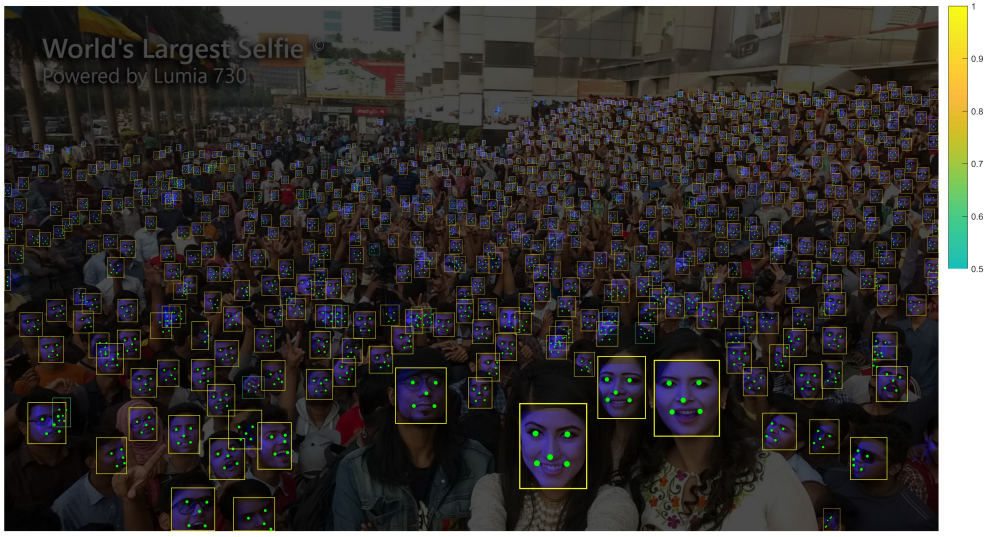
\includegraphics[width=0.85\textwidth]{figures/images/chapter-2/retinaface_example.png}
\caption{Qualitative example of face detection using RetinaFace in a crowded
real-world scene. Adapted from \cite{deng2020retinaface}.}
\label{fig:retinaface_example}
\end{figure}

RetinaFace also provides facial landmarks in addition to \gls{bounding box}es. The Figure~\ref{fig:retinaface_example} illustrates robust localization of many small and partially occluded faces. This supports downstream \gls{anonymization} steps where more precise localization is useful. RetinaFace was therefore selected as the face detector in \gls{SafeVision}.


\methodheading{PaddleOCR and Text Classification}

\gls{SafeVision} handles text-related \gls{anonymization} through a pipeline consisting of text detection, text recognition, and subsequent text classification. For text detection and recognition, the system uses PaddleOCR \cite{du2020ppocr}, which
provides an integrated \acrshort{ocr} framework for extracting textual content from natural images.

\begin{figure}[htbp]
\centering
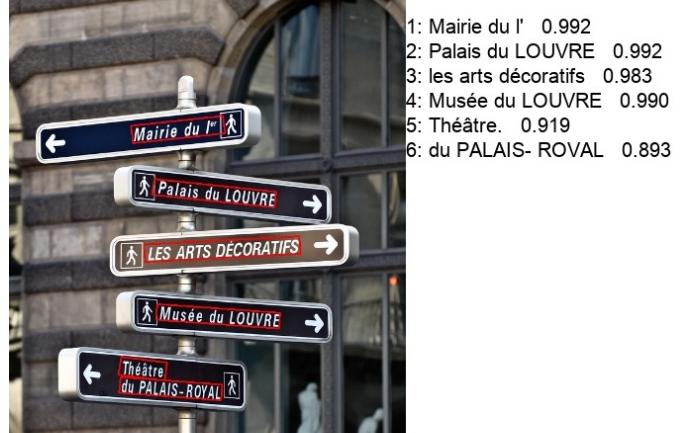
\includegraphics[width=0.70\textwidth]{figures/images/chapter-2/paddle_ocr_example.png}
\caption{Qualitative example of text detection and recognition using PaddleOCR
in a real-world scene. Adapted from \cite{du2020ppocr}.}
\label{fig:paddle_ocr_example}
\end{figure}

PaddleOCR was selected because it provides an end-to-end pipeline for localizing and recognizing text under varied visual conditions \cite{du2020ppocr}. This made it more suitable than generic \gls{object detection} alone, since text-based redaction depends on both identifying where text is located and extracting the content for further analysis.

After \acrshort{ocr}, the recognized text is further processed using a fine-tuned \acrshort{ner} model developed in this project, based on the XLM-RoBERTa base architecture \cite{conneau2020xlmroberta}. This was necessary 
because \acrshort{ocr} only extracts textual content, whereas selective redaction also  requires identifying which parts of the text belong to potentially sensitive entity categories. The combination of \acrshort{ocr} and \acrshort{ner}-based analysis therefore supports more selective and context-aware text redaction in \gls{SafeVision}.


\methodheading{\gls{yolox} for General and Custom Object Detection}

\Gls{object detection} in \gls{SafeVision} is based on \gls{yolox} \cite{ge2021yolox}. \gls{yolox} was selected because it combines strong detection performance with a simple and flexible framework for custom training. Its one-stage architecture makes it well suited for deployment and iterative experimentation.

\begin{figure}[H]
\centering
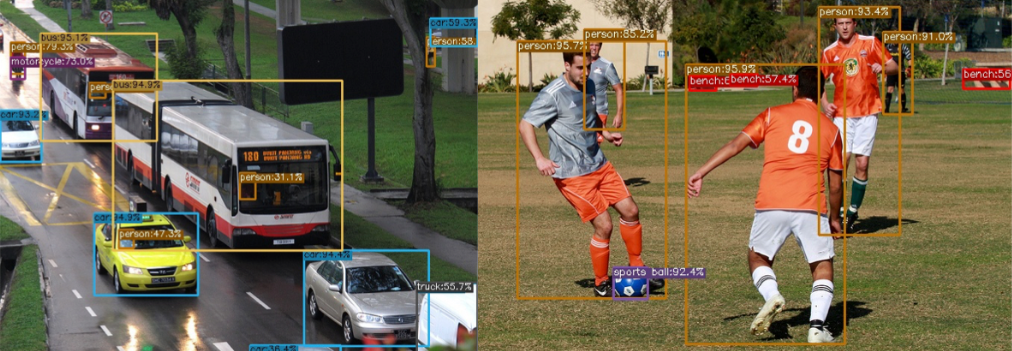
\includegraphics[width=\textwidth]{figures/images/chapter-2/yolox_example.png}
\caption{Qualitative example of \gls{object detection} using YOLOX. The figure illustrates localization of multiple object categories in natural scenes using \gls{bounding box}es and confidence scores. Adapted from \cite{yolox_github}.}
\label{fig:yolox_example}
\end{figure}

Within \gls{SafeVision}, \gls{yolox} is used in two different ways. First, existing \gls{yolox} models support detection of more general object categories relevant to the redaction workflow. Second, \gls{yolox} was used as the basis for custom-trained models targeting license plates and barcodes, where project-specific training was necessary. This made it possible to maintain a consistent detection framework while extending the system to object categories that were not sufficiently covered by the existing model setup.

The use of YOLOX also benefited from the availability of pretrained weights and well-documented training workflows in the official framework repository \cite{yolox_github,ge2021yolox}. This reduced training time and made it feasible to develop custom object detectors within the constraints of the project.


\methodheading{Video Processing and Tracking in \gls{SafeVision}}
\phantomsection
\label{sec:video_tracking_foundation}

\gls{SafeVision} handles video as a sequence of frames, where \gls{anonymization} must remain temporally consistent across time rather than being treated as a set of independent image outputs. For this reason, the system combines frame-level detection with tracking.

At user selected frames, \gls{SafeVision} applies the same detection pipeline used for still images. Between such frames, tracking is used to propagate and stabilize sensitive regions across consecutive frames, which reduces the need for repeated full detection and helps maintain visually consistent \gls{anonymization}.

For AI-generated detections, \gls{SafeVision} uses a multi-object tracking approach based on \gls{kalman filter}ing and entity specific association across frames \cite{bewley2016sort}. The tracker predicts \gls{bounding box}es over time and matches new detections to existing tracks using a combination of \gls{intersection over union} (\acrshort{iou}) and motion consistency. It also maintains track history and supports interpolation across detection gaps, which makes it
possible to backfill intermediate frames when detections are temporally sparse. 

For manually selected regions, \gls{SafeVision} uses a dedicated object-tracking component based on OpenCV tracking methods. The implementation prioritizes the ViT tracker from OpenCV Zoo when the required tracker implementation and ONNX model are available, because it provides a modern deep-learning-based tracking approach suitable for following user-defined objects across frames. Channel and Spatial Reliability Tracking (\acrshort{csrt}) is retained as a fallback because it is widely available in OpenCV and provides a practical conventional tracker when the ViT tracker cannot be used \cite{opencv_vittrack, lukezic2017csrt}. Manual tracking is applied forward and backward from the selected frame, allowing a user-defined \gls{bounding box} to be propagated through the surrounding sequence. Additional safety checks are used to detect unstable tracker output, including low confidence, implausible changes in size or aspect ratio, large center jumps, and weak overlap with the last trusted region.

\methodheading{\Gls{segmentation} and \Gls{inpainting} for Redaction Refinement}
\label{subsec:segmentation-and-inpainting-for-redaction-refinement}

To improve redaction quality beyond coarse \gls{bounding box} \gls{masking}, \gls{SafeVision} also includes refinement components for \gls{segmentation} and region replacement. For \gls{segmentation}, the system uses \gls{mobilesam} \cite{mobilesam}, a lightweight \gls{segmentation} model derived from the Segment Anything approach
\cite{kirillov2023segment}, in order to produce more precise masks for selected regions before redaction is applied.

\begin{figure}[H]
\centering
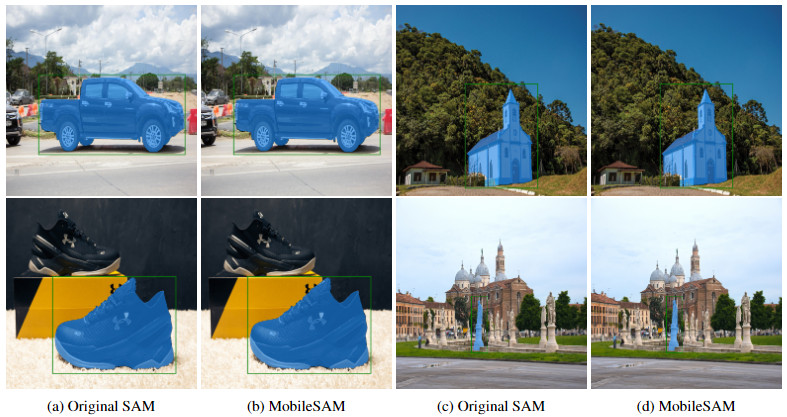
\includegraphics[width=0.8\textwidth]{figures/images/chapter-2/mobile_sam.png}
\caption{Comparison between \gls{segmentation} results produced by the original Segment Anything Model (\acrshort{sam})
and \gls{mobilesam}. The examples illustrate that \gls{mobilesam} can provide similar object masks while using a more lightweight model. Adapted from \cite{mobilesam}.}
\label{fig:mobile_sam}
\end{figure}

\gls{mobilesam} was selected to support more precise redaction where rectangular \gls{bounding box}es would include too much surrounding visual content. It enables more selective \gls{anonymization} than \gls{bounding box}-based redaction while remaining easier to integrate than heavier \gls{segmentation} models. Its compact size was also an important consideration, since \gls{SafeVision} is developed as a web application where lightweight and deployable components are preferable.

\begin{figure}[H]
\centering
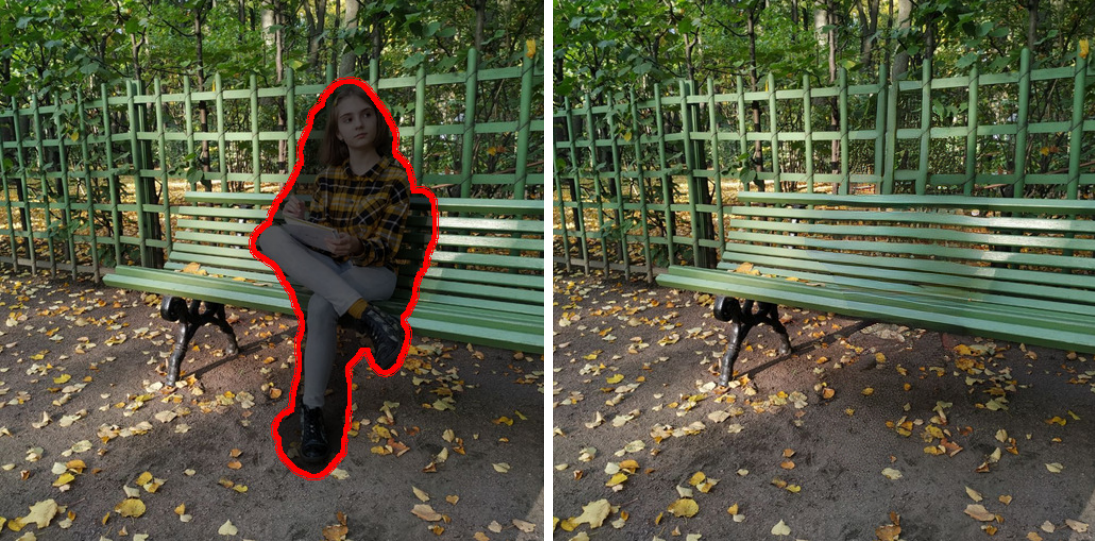
\includegraphics[width=0.7\textwidth]{figures/images/chapter-2/inpaint.png}
\caption{Illustration of image \gls{inpainting}, where a selected region is replaced
with generated background content instead of being masked directly. Adapted from
\cite{rombach2022high}.}
\label{fig:inpaint_example}
\end{figure}

For region replacement, the system uses a Stable Diffusion \gls{inpainting} model based on the \texttt{runwayml/stable-diffusion-inpainting} checkpoint \cite{sd_inpaint_model,rombach2022high}. This allows selected regions to be replaced with generated content instead of being blurred or masked directly. \Gls{inpainting} was nevertheless treated as a complementary refinement method rather than the default strategy, since visually cleaner output does not necessarily produce a more reliable form of \gls{anonymization}.


\methodheading{Why Hybrid User Review Was Retained}
\label{sec:why_hybrid_user_review_was_retained}

Although \gls{SafeVision} uses several strong AI-based components, the system was not designed as a fully autonomous redaction pipeline. Automated approaches still face practical limitations related to missed detections, \gls{false positive}s, and
context-dependent cases \cite{orekondy2017connecting, zhao2023visual}. User review was therefore retained as a central design principle in \gls{SafeVision}. Automatic detection reduces manual workload, while the user remains able to inspect, modify, and approve the final result before redaction is completed. This reduces reliance on fully automated decisions in cases where mistakes may expose sensitive information.

\section{Synthesis and Design Implications}

The reviewed theory and methods show that visual redaction requires a multi-component approach. Faces, embedded text, structured objects, and irregular regions differ in how they must be detected, interpreted, and anonymized. This motivated the use of specialized components in \gls{SafeVision}, rather than a single general-purpose model.

For video, this also introduces a temporal requirement: sensitive regions must be handled consistently across consecutive frames, which motivates the use of tracking mechanisms in addition to frame-level detection.

The review also shows that fully automated redaction remains limited by \gls{false negative}s, \gls{false positive}s, and context-dependent privacy risks. \gls{SafeVision} was therefore designed as a hybrid system: automated detection reduces manual work, while user review preserves control over the final anonymized output. These implications shaped the system requirements, architecture,
implementation, and evaluation presented in the following chapters.


\afterpage{\blankpage}
